\documentclass{beamer}

\usepackage{hyperref}

\usepackage{array}
\usepackage{setspace} 
\usepackage{graphicx}
\usepackage[utf8]{inputenc}
\usepackage[croatian]{babel}
\usepackage{amsmath}
\usepackage{xfrac}
\usetheme{Singapore} 
\title[Statistički praktikum 1 - 36. zadatak]{Statistički praktikum 1 - 36. zadatak}
\author{Hermina Petric Mareti\'{c}}

\setstretch{1.25}

\begin{document}

\begin{frame}
\titlepage
\end{frame}

\begin{frame}{Opis zadatka}
\begin{itemize}
\item List indijanske penjačice može biti šaren ili jednoličan, te istovremeno blijed ili
normalne boje. 
\item Postavljeno je pitanje jesu li te dvije karakteristike nezavisne. 
\item Prijašnji eksperimenti su pokazali da će mladica s
vjerojatnosti $\sfrac{1}{4}$ biti blijeda (a normalne boje s vjerojatnosti $\sfrac{3}{4}$ ). Isto tako lišće mladica ce s
vjerojatnosti $\sfrac{1}{4}$ biti šareno (a s vjerojatnosti $\sfrac{3}{4}$ jednolično). 
\item Na slučajan način prikupljen je
uzorak od 290 mladica indijske penjačice.
\end{itemize}
\begin{center}
\begin{tabular}{|c|c|c|}
\hline 
 & normalne boje & blijedo \\ 
\hline 
jednolično & 187 & 35 \\ 
\hline 
šareno & 37 & 31 \\ 
\hline 
\end{tabular} \\
\end{center}
\end{frame}

\begin{frame}{(a) zadatak}
\begin{itemize}
\item Neka je X stanje prve karakteristike (šareno ili lišće jednolične boje), a Y stanje druge
karakteristike (blijedo lišće ili normalne boje). 
\item Na osnovi danog uzorka, procijenite zajedničku
razdiobu varijabli X i Y, tj. procijenite razdiobu vektora (X,Y) i grafički je predstavite.
\item Također, graficki je usporedite s razdiobom u kojoj su X i Y nezavisne, a marginalne razdiobe
su u skladu s prijašnjim saznanjima.
\end{itemize}
\end{frame}

\begin{frame}{Razdioba vektora (X,Y)}
\begin{center}
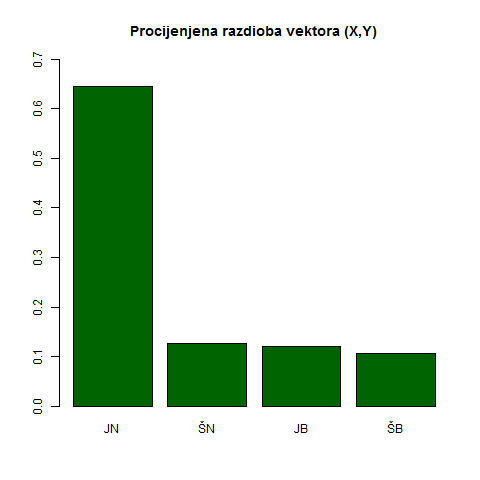
\includegraphics[scale=0.35]{1.png}\\
\end{center}
\end{frame}

\begin{frame}{Usporedba procijenjene i nezavisne razdiobe}
\begin{center}
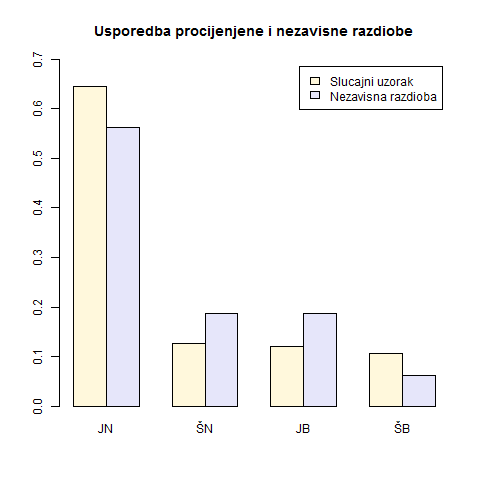
\includegraphics[scale=0.35]{2.png}\\
\end{center}
\end{frame}

\begin{frame}{(b) zadatak}
\begin{itemize}
\item Testirajte da li su X i Y nezavisne s pretpostavljenim marginalnim razdiobama kao u
tekstu zadatka.
\item Postavljamo hipoteze:\\
\item $ H_{0} $= X i Y su nezavisne s pretpostavljenim marginalnim razdiobama\\
\item $ H_{0} $= X i Y nisu neazavisne s pretpostavljenim marginalnim razdiobama\\
\item Za testiranje koristimo Pearsonov $\chi^2$-test o pripadnosti distribuciji s testnom statistikom 
$H=\sum_{i=1}^{r} \sum_{j=1}^{c} \dfrac{(f_{i,j}-f_{i,j}')^2}{f_{i,j}'} \sim \chi^2(r*c-d-1)$
\end{itemize}
\end{frame}

\begin{frame}{(b) zadatak}
\begin{itemize}
\item Kritično područje: $[7.815,\infty\rangle$
\item Vrijednost testne statistike: h=25.096 
\item Odbacujemo nultu hipotezu na razini značajnosti od 5\% 
\item P-vrijednost: $1.47*10^{-5}$ 
\end{itemize}
\end{frame}

\begin{frame}{(c) zadatak}
\begin{itemize}
\item Odredite jakost testa iz (b) uz značajnost 5\%
\item Postavljamo hipoteze:\\
\item $H_{0}: p=p^{(0)}$\\
\item $H_{1}: p=p^{(0)} - \frac{1}{\sqrt{n}} \delta$, za neki $\delta\neq 0$\\
\end{itemize}
\end{frame}

\begin{frame}{(c) zadatak}
\begin{itemize}
\item Testna statistika je $H=\sum_{i=1}^{r} \sum_{j=1}^{c} \dfrac{(f_{i,j}-f_{i,j}')^2}{f_{i,j}'} \sim \chi^2(r*c-d-1)$\\
\item Ako vrijedi hipoteza $H_{1}$, tada je $H\sim A_{\chi^2} (k-1,\lambda)$, gdje je $\lambda=\sum_{k=1}^k \dfrac{\delta_{i}^2}{p_{i}^0}$ parametar
necentralnosti.\\
\item Tada funkciju jakosti Pearsonovog $\chi^2$-testa možemo prikazati ovako:\\
$\gamma(\lambda)=P(H\geq \chi^2(k-1)|p=p^0-\frac{1}{\sqrt{n}}*\delta)=1-P_{\chi^2(k-1,\lambda)}(\chi_{\alpha}^2 (k-1))$\\
\end{itemize}
\end{frame}

\begin{frame}{(c) zadatak}
\begin{center}
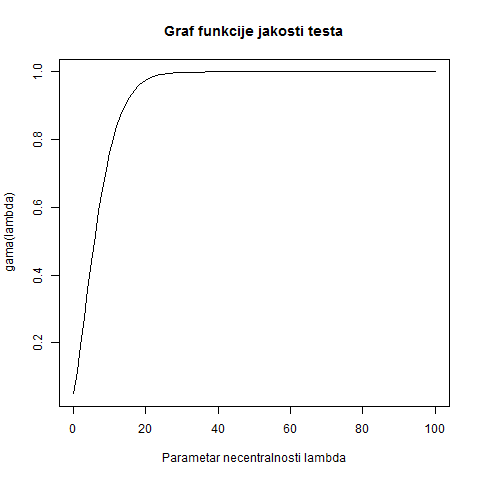
\includegraphics[scale=0.27]{3.png}\\
\end{center}
\begin{itemize}
\item Minimum se postiže u točki 0 i iznosi 0.05. To proizlazi iz činjenice da hipoteza $H_{0}$ govori upravo da je $\lambda=0$ i iz činjenice da test ima razinu značajnosti 5\%.\\
\end{itemize}
\end{frame}

\begin{frame}{(d) zadatak}
\begin{itemize}
\item Prema jednoj drugoj teoriji, razdioba od (X,Y) je oblika\\
\begin{center}
\begin{tabular}{|c|c|c|}
\hline 
X \ Y & normalne boje & blijedo \\ 
\hline 
jednolično & $\sfrac{9}{16} + \theta $ & $\sfrac{3}{16} - \theta $ \\ 
\hline 
šareno & $\sfrac{3}{16} - \theta $ & $\sfrac{1}{16} + \theta $ \\ 
\hline 
\end{tabular} \\
\end{center}
gdje je H nepoznati parametar. Odredite parametarski prostor i pomoću 
$ \chi ^2$-testa testirajte
tu hipotezu, pri čemu nepoznati parametar procjenite minimum $ \chi ^2$-metodom.
\end{itemize}
\end{frame}

\begin{frame}{(d) zadatak}
\begin{itemize}
\item Parametarski prostor: $\theta \in [\sfrac{-1}{16}, \sfrac{3}{16}]$
\item Minimum $\chi^2$-metoda se temelji na tome da za funkciju $h(\theta):\Theta\rightarrow R$, $h(\theta)=\sum_{i=1}^{k} \sum_{j=1}^{c} \dfrac{(f_{i,j}-f_{i,j}'(\theta))^2}{f_{i,j}'(\theta)}$ tražimo vrijednost $\hat{\theta}$ u kojoj ona postiže minimum.
\end{itemize}
\end{frame}

\begin{frame}{(d) zadatak}
\begin{center}
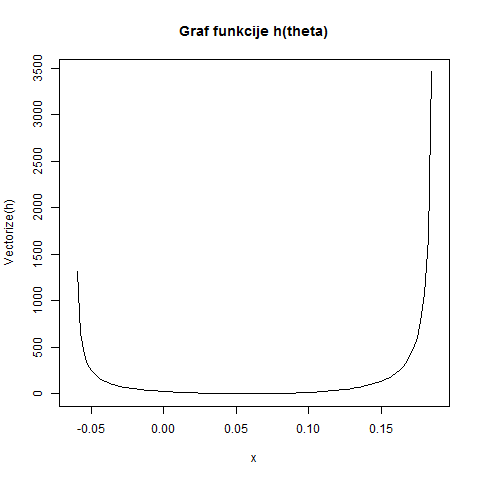
\includegraphics[scale=0.28]{4.png}\\
\end{center}
\begin{itemize}
\item Kao što i otprilike vidimo na grafu, minimum se postiže u točki 0.0586, pa je baš to naš $\hat{\theta}$. \\
\end{itemize}
\end{frame}

\begin{frame}{(d) zadatak}
\begin{itemize}
\item Testiramo hipotezu da je razdioba našeg slučajnog vektora iz zadanog modela
\item Iskoristimo procijenjeni parametar $\theta$ i provodimo $\chi^2$-test s 2 (d=1 jer imamo jedan procijenjeni parametar) stupnja slobode. 
\item P-vrijednost: 0.6371446
\item P-vrijednost je velika, pa ne možemo odbaciti hipotezu o pripadnosti zadanom modelu.\\
\end{itemize}
\end{frame}

\begin{frame}{(e) zadatak}
\begin{itemize}
\item Procijenite nepoznati prametar iz modela u (d) metodom maksimalne vjerodostojnosti
i usporedite ga s minimum $ \chi ^2$-procjenom
\item Definiramo funkciju vjerodostojnosti $L:\Theta \rightarrow R$, sa $L(\theta)=\prod_{i=1}^{n} f(x_{i}|\theta)$. Tražimo $\theta$ koji maksimizira ovu funkciju i zovemo ga procjenom metodom maksimalne vjerodostojnosti.
\end{itemize}
\end{frame}


\begin{frame}{(e) zadatak}
\begin{center}
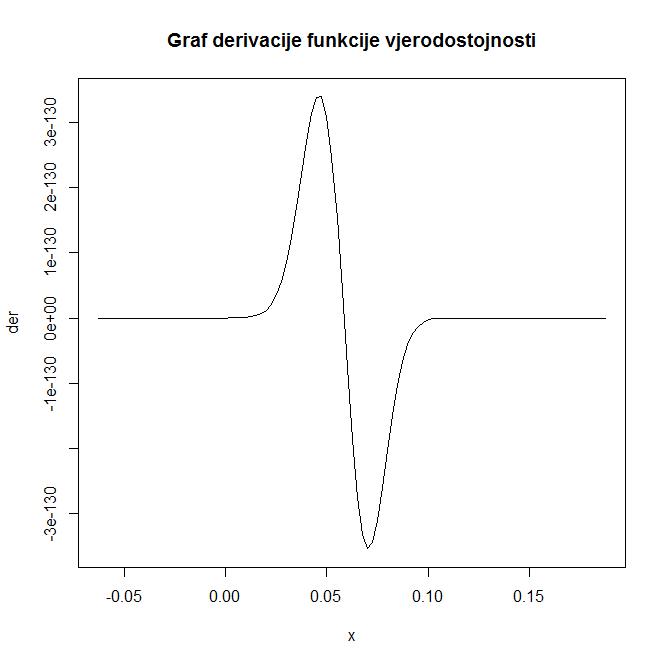
\includegraphics[scale=0.25]{5.png}\\
\end{center}
\begin{itemize}
\item $\hat{\theta} = 0.05840407$
\end{itemize}
\end{frame}


\begin{frame}{(e) zadatak}
\begin{center}
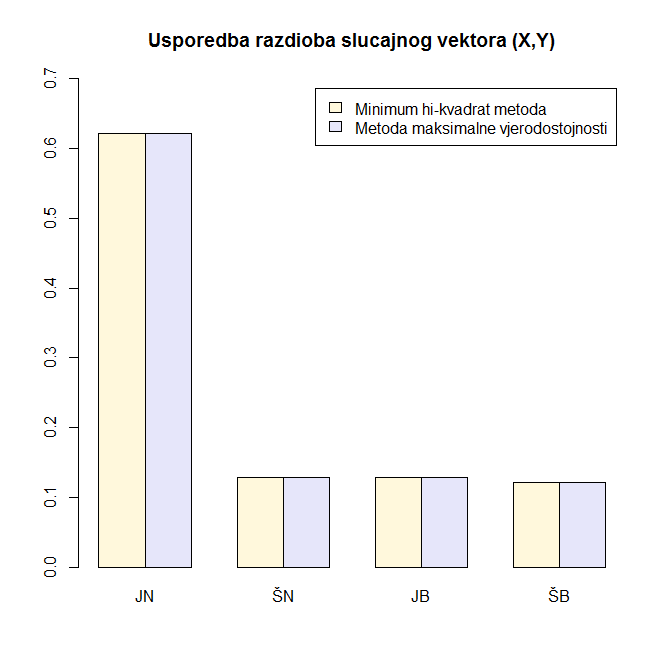
\includegraphics[scale=0.25]{6.png}\\
\end{center}
\end{frame}

\begin{frame}
\begin{center}
Hvala na pažnji!
\end{center}
\end{frame}

\end{document}
